\section{Context}\label{context}

Biogeographers are still debating about if the biotic interactions at
the local scale impact large scale species distribution. If this is
indeed the case, then we should expect pairs of species to exhibit
non-random distribution at the large spatial scale. In order to test
whether interactions influence species distributions, the simplest
avenue is to investigate species co-distribution in light of their
ecological relationships. Such investigation started with Diamond's
original study stating that species interacting by competition should
avoid each other in space, leading to a `checkerboard' distribution
\citep{Diamond1975}. This idea was rapidly criticized for the lack of an
adequate null hypothesis \citep{Connor1979, Gilpin1982} and has led to
an historical controversy \citep{Hutchinson1959}. Nowadays, the observed
co-distribution is compared to the co-distribution expected under random
distribution, and strong significant associations (either positive or
negative) are interpreted as evidence of ecological interactions.

Species ranges are very often inferred from the realized distribution,
which result from the joint impacts abiotic and biotic environmental
factors along with dispersal limitations and historical contingencies
\citep{Pulliam2000, Holt2009, Araujo2014}. Finding evidence of the
effect of species interactions on distribution may prove technically
difficult, which would explain the scarcity of studies reporting such
effect (but see \citet{Gotelli2010}). Fortunately, recent developments
in co-occurrence theory promises novel avenues in which highly
dimensional species distribution data could be analyzed, accounting for
the structure of the network of ecological interactions
\citep{Cazelles2016}. It formalized the interpretation of fundamental
and realized niches based on conditional and marginal occurrence
probabilities (Box 1). Further, it proposed several testable
predictions, including that the higher the degree of a species,
\emph{i.e} the number of species which with it interacts, the weaker
will be the detection of a signal of co-occurrence. Finding good
correspondence between network topology and species associations in
empirical data would support the idea that interactions affect
geographic ranges, even if for many pairs of interacting species no
significant co-occurrences are found.

Despite the fantastic number of studies investigating co-occurrence in
order to understand community assembly, the hypothesis that species
interactions should result in non-random associations in space has never
been tested formally. It is rather implicitly assumed in every
investigation. Our objective in this study is therefore to test this at
the scale of species range. We analyzed species association within five
different datasets ranging from plant-seed dispersers, host-parasitoids,
microbes, birds and forest trees. We quantify conditionnal co-occurrence
for species that are known to interact and known to not interact
directly. We report no difference between pairs of interacting species
and pairs of not-interacting species. However our results suggest that
the degree of a species in a network influences our ability to detect
significant associations. Moreover, we discover a clear relationship
between the strength of species associations and the cumulated occupancy
of the entire set of species with which a species interact.

\section{Material and Methods}\label{material-and-methods}

\subsection{Datasets}\label{datasets}

We analyzed five datasets spawning a large range of organsim and types
of interactions (see \citet{tbl:id}), across an extensive gradient of
environmental conditions (see Fig S1 and SI Text). Our criteria for
selecting datasets were as follow: i) the occurrence data must have been
collected at the local scale, it could not be derived from range maps;
ii) data included observed absences; iii) occurrence was observed for
all species, not only a singe layer; interactions were known a priori;
v) since we are computing co-occurrences, which is typically a fairly
rare event, we needed an elevated number of sampling units. Direct
interactions were documented for four datasets and represented by
networks of ecological interactions: the Willow Leaf Network (WLN), the
Pitcher Plants Network (PPN), the Caribbean Hummingbirds Network (CHN),
the French Breeding Birds Survey (FBBS). We derived metawebs for each
network, \emph{i.e}, the matrix recording all interactions, and computed
three metrics among species from a regional pool: the connectance of
metawebs (proportion of realized interactions), the degree of species
(number of links for one species) and the shortest-path between all
pairs of species (the minimum number of link from one species to the
other, see SI Text). For the North American Trees (NAT) dataset, we
approximated competitive interactions by computing functional distance
between every pair of species (see table S1 and Fig S2). Similar proxy
for ecological interactions was also computed for the FBBS see table
S2). Only species that were present at least on 1\% of the total number
of observations were considered for the analysis (see SI Text).

\subsection{Quantifying co-occurrence}\label{quantifying-co-occurrence}

For each pair of species \(i\) and \(j\) we computed the number of
observed co-occurrence \(O_{i,j}\) and the expected number of
co-occurrence under independent distribution \(E_{i,j}\). Standard
deviation \(SD_{i,j}\) We report the Z-score
\(O_{i,j}-E_{i,j}/SD_{i,j}\) \citep{Gilpin1982}, a standardized metric
of co-occurrence, with positive (negative) values indicating more (less)
co-occurrence relative to the random expectation. Expectations were
derived using three different methods. First, we assumed that all sites
were equivalent, meaning we ignored the potential influence of abiotic
conditions across the entire range. The observed co-occurrence is an
estimate computed from a limited number of observations
\citep{Gilpin1982, Veech2013} and therefore, we also considered an
hypergeometric distribution, which corrects for limited sample size (see
SI Text for further details). We used two different SDMs in order to
account for the abiotic environment and correct the random expectation,
namely, Generalized Linear Model (hereafter GLM) and Random Forest
(hereafter RF - see SI Text for more details and Fig S3 for the
assessment of models' performances). The correction using SDMs accounts
for the fact that species may co-occur simply because they have similar
abiotic requirements, irrespective of if they interact or not.

\section{Results}\label{results}

We observed a clear difference in the strength of spatial associations
between interacting and not-interacting species (\ref{fig:synth} panels
A to D) for two out of four datasets for which direct interactions were
known. In all cases, spatial associations were positive, indicating that
interacting species are co-occurring more often that expected by chance,
irrespective of the type of interaction. \% DG: what do you mean with
the following sentence ? That if you do a C-Score you would not detect
associations ? Therefore, when integrating all pairs of species we did
not obtain a clear evidence that direct interaction species co-occur
differently from not-interacting one. For the WLN, distinguishing
herbivore-willow interactions from herbivore-parasitoids revealed that
the strength of co-occurrence was stronger for the former than the
latter ones (\ref{fig:shtpth} A-B). Interestingly, we noticed that the
higher the mean degree of species in the dataset, the more difficult the
detection of a signal of interactions in co-occurrence was
(\ref{fig:shtpth} A-D).

We observed that the strength of spatial association was higher for
pairs of similar species (\ref{fig:synth} panels E and F) for the NAT
and FBBS datasets, for which we inferred a distance based on functional
traits. Functional similarity is often interpreted as a proxy for
competition strength \citep{Morales-Castilla2015}, which would suggest
that competition is poorly detectable at large scale which is
theoretically supported \citep{Araujo2014}. Interestingly however, the
spatial association was positive, which is at the opposite of Diamond's
hypothesis of the consequences of competition on spatial distribution.
Therefore, co-occurrences of similar species are likely driven by the
similarity of their abiotic requirements. The results for the FBBS
dataset were identical irrespective the type of traits examined (Fig
S4). This hypothesis was further supported by the decrease of the
Z-score with the distance for both datasets (fig S6 A and D).

For all datasets, we report that the distribution is concentrated but
the Wilcoxon rank test we used (see SI Text) lead us to the distribution
is symmetric about 0 taking environmental context into account shifts
the distribution toward 0 and diminishes the variance associated
(\ref{fig:synth}). This trend is more pronounced for RF than for SDM.
Hence, assuming that sites are not identical for species due to the
abiotic context reduces the signal of co-occurrence which could even
disappeared. In the PPN dataset, we found that the signal is even
reversed (\ref{fig:synth}) but the quality of the SDM approaches used
were low (fig S3 B).

We investigated if the strength of associations between species
interacting indirectly decreases with the shortest path length between
them.

Co-occurrence was not different from random distribution for pairs of
species that are only interacting indirectly (shorthest path length
­\textgreater{} 1) - \ref{fig:shtpth} A-D) as predicted by the theory,
but the observed decay was steeper than anticipated
\citep{Cazelles2016}. The decay is similar when all pairs of species
were taken into account (see Fig S5). Moreover when we calculated the
mean degree in of predators (pollinators), we also found for predators
and poolinations that the signal of co-occurrence for low shortest path
is stronger for specialists (\ref{fig:shtpth} A) than for generalists
(\ref{fig:shtpth} C), suggesting that the abundance of interactions may
prevent us from detecting them in static occurrence data.

Finally, we analyzed the mean Z-score of a predator (pollinator),
\emph{i.e} Z-scores averaged over all the set of its preys (host
plants), against the total number of site covered by its preys (hots)
(\ref{fig:degocc}). We report that when abiotic context is not taken
into account, their is a clear negative relationship explaining up to
.69 of the variance (\ref{fig:degocc} panels A, D, G and J). Therefore,
when a predator feeds on a set of preys that jointly cover a large part
of the geographic range studied, the impact of species interactions is
undetectable, but when the joint repartition of the prey is restricted,
the imprint of interactions remains appreciable. Additionally, the
associated linear regression outperformed the one using the degree of
the species that has been envisioned by the theory (Fig S7 panels A, D,
G and J). Also, we show this relation asymmetric: the decay is less
convincing when the the mean Z-scores of the preys are plotted against
the cumulated range of their predators (fig S8 panels A, D, G and J).
Hence the imprints of interactions in static occurrence are appreciated
once relevant pair of specials species are student. When species are
highly linked with other species and when these species have ranges that
do not completely overlap, we cannot make clearly co-occurrence to
interactions. This suggest that the range of the set of species should
be examined rather that individual range of prey. Interestingly, we
found that using the presence of the whole set of prey as predictor to
assign the presence of species outperformed GLMs (see Fig S9) but not
RFs.

All these last results are no longer true once abiotic constrains are
taken into account, the clear relationship obtained is either weakened
or even reversed (\ref{fig:degocc} B,C,E,F,H,I,K,L) meaning the signals
of co-occurrence for specialists are no longer different from the one of
generalists. If we consider that this relationship is biologically
meaningful as biotic constraints may be softer for generalists than for
specialists we must then question to what extent inferring species
distribution fail in capturing occurrence properties exhibit by species
assemblage.

\subsection{Discussion}\label{discussion}

Our study demonstrate how information on ecological interactions can
shed light upon distribution over broad spatial scales. Although we
reject the hypothesis that interacting species co-occur differently from
non-interacting one once accounting for the abiotic environment, we
highlight the possibilities offer by asking alternative questions such
as the impact of the abundance of interactions and the relative
positions of two species within the network on their co-occurrence. Our
results demonstrate that there is an imprint of ecological interactions
on occurrence data but also that there are specific conditions under
which they can be detected. Hence, we find that the signal of
co-occurrence is blurred by the number of interactions a species
experience, in agreement with recent co-occurrence theory
\citep{Cazelles2016}. As a consequence, the distribution of a given
species is more strongly related to the distribution of the entire set
of species it interacts with, than each species thaken individually.
This indicates that the role of ecological interactions may not only be
a matter of spatial scale \citep{McGill2010}, but also a matter of
picking the most consistent biological unit to investigate distribution
over large spatial scales.

Species distribution models are based on the assumption that species are
distributed independently from each other and that scenarios of
tomorrow's biodiversity can be anticipated using abiotic variables only
\citep{Jeschke2008}. Some recent developments in statistics relaxed this
hypothesis by representing the distribution of assemblages, based on
correlations between species \citep{Pollock2014, Warton2015b}. The
development of these powerful statistical tools is essential, however it
can only provide a partial solution to some limitations of SDms.\\
A substantial part of the solution lies in the understanding of the role
of ecological and evolutionary mechanisms shaping distributions
\citep{Thuiller2013}. Here, we underline the need for not hypothesizing
\emph{a priori} the independence among species. Rather, the assumption
must be proved to apply, otherwise a relevant assemblage must be
modeled. We suggest that for generalist species, the assumption of
independence is reasonable while for specialists the relative position
with the other species within the network should help deciding which set
of species are to be modeled. We therefore suggest that a priori
information on ecological interactions should be integrated in SDMs The
integration of information should greatly strengthen our predictions for
a fair additional complexity into our SDMs.

Our results lead us to conclude that co-occurrence tends to the
independence with increasing diversity of interactions. Only the
specialized species are strongly associated with their partners, as
generalists experience a much more diffuse constraint from interacting
speceis.\\
Similarly, it it has been recently highlighted that net species
interaction strength better pairs of species is better predicted when
the species richness increases \citep{Berlow2009}. Further, press
perturbations applied to specialist species do have much stronger
indirect impacts on the other species than perturbations applied to
generalists (Montoya2009). All of these results are congruent with
MacArthur's vision, who more than 40 years ago, noticed the following
paradox \emph{``How can a more complex community be easier to
understand? A possible answer might be that the complex community have
strong interactions among species so that the lives of the separate
species are less independent than in a simple community. Where there is
greater interdependence, patterns may be more conspicuous.''}
\citep[p.199]{macarthur1972geographical}. In our study, the strong
interactions among species ease the forecasting of species distribution.
However, under the ongoing mass extinction, a myriad of links vanishes
while new ones emerge with the changes in the composition of local
communities. Therefore, even if under current conditions the assumption
of independence may be valid, under dramatic modifications of ecosystem
as currently observed, it may often prove false. As a step forward, new
biodiversity scenarios must not solely map the future ranges of
individual species but the entire community including the consequences
of potential extinction on community structure.

\newpage

\subsection{Box 1}\label{box-1}

The fundamental niche is here defined as the occurrence probability
under the assumptions that (1) biotic factors are not limiting occupancy
and (2) that dispersion is unlimited. In this case, only abiotic factors
(such as water availability, temperature variability and edaphic
variables) limit survival and/or reproduction success, and then the
occurrence probability. Consequently, predator occupancy is represented
under the assumtion that preys are abundant enough all along the
environmental gradient. Similarly, the fundamental niche of any prey is
not influenced neither by predators nor by its competitors.

For a three species network made of one predator and two preys, we
consider the three fundamental niches \(f_i\) (\ref{fig:box1} A). We
consider preys are substituable and the presence of at least one prey is
sufficient to sustain the predator:

\[f_3(w)=P(X_3=1|X_2+X_1>0, G=w)\]

where \(G\) denotes the environmental gradient and \(X_i\) is the random
variable associated to the presence of species \(i\). Similarly, \(f_1\)
and \(f_2\) are obtained assuming that 3 is absent :

\[f_2(w)=P(X_2=1|X_3=0, G=w)\]

and:

\[f_1(w)=P(X_1=1|X_3=0, G=w)\]

Once projected on a map, the fundamental niche unravels the potential
distribution of a species \citep{Kearney2004}.

The expected distribution can be compared to real observations and could
reveal whether dispersal limits and ecological interactions are
prevalent in the occupancy dynamic of studied species. The realized
niche (\ref{fig:box1} B) includes these factors.\\
In our simplified example, fundamental and realized niches of preys are
identical. The realized niche of the predator, \(r_3\), is constrained
by the joint realized niches of its preys:

\[r_3(w)=f_3(w)\left(1-(1-r_1(w))(1-r_2(w))\right)\]

The above expression may often be more complicated due to the size and
the structure of the interaction network. For instance, we do not
consider the apparent competition between species 1 and 2, although it
must affect their co-distribution. Integrating the impact of many
interactions may be possible using occurrence probabilities of species
assemblages rather than single species \citep{Cazelles2015b}.

Integrating network information to shed light upon species distribution
is also crucial to understand what circumstances where co-occurrence
will be meaningful. Consider as an example the co-occurrence between
species 1 and 3: the co-occurrence may be strong if we restrict the
analysis to the suitable conditions for species 1 {[}GIVE THE RANGE ON
THE FIGURE {]} but it must be weak if the entire environmental gradient
is sampled. However, if we examine the co-occurrence between 3 and the
assemblage made of species 1 plus 2, the co-occurrence will always be
strong. Although this is meaningful from a biological point of view,
co-occurrence studies often remain focus on pairs of species.

\newpage

\subsection{Tables}\label{tables}

\begin{longtable}[]{@{}lrrrrrrr@{}}
\caption{Data sets analyzed in this article.
\label{tbl:data}}\tabularnewline
\toprule
\begin{minipage}[b]{0.15\columnwidth}\raggedright\strut
Type\strut
\end{minipage} & \begin{minipage}[b]{0.07\columnwidth}\raggedleft\strut
No. of sites\strut
\end{minipage} & \begin{minipage}[b]{0.07\columnwidth}\raggedleft\strut
No. of species\strut
\end{minipage} & \begin{minipage}[b]{0.11\columnwidth}\raggedleft\strut
Interaction type\strut
\end{minipage} & \begin{minipage}[b]{0.05\columnwidth}\raggedleft\strut
Observed\strut
\end{minipage} & \begin{minipage}[b]{0.04\columnwidth}\raggedleft\strut
Traits\strut
\end{minipage} & \begin{minipage}[b]{0.06\columnwidth}\raggedleft\strut
Connectance\strut
\end{minipage} & \begin{minipage}[b]{0.22\columnwidth}\raggedleft\strut
References\strut
\end{minipage}\tabularnewline
\midrule
\endfirsthead
\toprule
\begin{minipage}[b]{0.15\columnwidth}\raggedright\strut
Type\strut
\end{minipage} & \begin{minipage}[b]{0.07\columnwidth}\raggedleft\strut
No. of sites\strut
\end{minipage} & \begin{minipage}[b]{0.07\columnwidth}\raggedleft\strut
No. of species\strut
\end{minipage} & \begin{minipage}[b]{0.11\columnwidth}\raggedleft\strut
Interaction type\strut
\end{minipage} & \begin{minipage}[b]{0.05\columnwidth}\raggedleft\strut
Observed\strut
\end{minipage} & \begin{minipage}[b]{0.04\columnwidth}\raggedleft\strut
Traits\strut
\end{minipage} & \begin{minipage}[b]{0.06\columnwidth}\raggedleft\strut
Connectance\strut
\end{minipage} & \begin{minipage}[b]{0.22\columnwidth}\raggedleft\strut
References\strut
\end{minipage}\tabularnewline
\midrule
\endhead
\begin{minipage}[t]{0.15\columnwidth}\raggedright\strut
Willow Leaf Network\strut
\end{minipage} & \begin{minipage}[t]{0.07\columnwidth}\raggedleft\strut
374\strut
\end{minipage} & \begin{minipage}[t]{0.07\columnwidth}\raggedleft\strut
156\strut
\end{minipage} & \begin{minipage}[t]{0.11\columnwidth}\raggedleft\strut
Trophic / Parasitism\strut
\end{minipage} & \begin{minipage}[t]{0.05\columnwidth}\raggedleft\strut
yes\strut
\end{minipage} & \begin{minipage}[t]{0.04\columnwidth}\raggedleft\strut
no\strut
\end{minipage} & \begin{minipage}[t]{0.06\columnwidth}\raggedleft\strut
0.042\strut
\end{minipage} & \begin{minipage}[t]{0.22\columnwidth}\raggedleft\strut
unpublished\strut
\end{minipage}\tabularnewline
\begin{minipage}[t]{0.15\columnwidth}\raggedright\strut
Pitcher Plants Network\strut
\end{minipage} & \begin{minipage}[t]{0.07\columnwidth}\raggedleft\strut
39x20\strut
\end{minipage} & \begin{minipage}[t]{0.07\columnwidth}\raggedleft\strut
53\strut
\end{minipage} & \begin{minipage}[t]{0.11\columnwidth}\raggedleft\strut
Trophic\strut
\end{minipage} & \begin{minipage}[t]{0.05\columnwidth}\raggedleft\strut
yes\strut
\end{minipage} & \begin{minipage}[t]{0.04\columnwidth}\raggedleft\strut
no\strut
\end{minipage} & \begin{minipage}[t]{0.06\columnwidth}\raggedleft\strut
0.44\strut
\end{minipage} & \begin{minipage}[t]{0.22\columnwidth}\raggedleft\strut
\citet{Baiser_2011}\strut
\end{minipage}\tabularnewline
\begin{minipage}[t]{0.15\columnwidth}\raggedright\strut
Caribbean Hummingbirds Network\strut
\end{minipage} & \begin{minipage}[t]{0.07\columnwidth}\raggedleft\strut
32\strut
\end{minipage} & \begin{minipage}[t]{0.07\columnwidth}\raggedleft\strut
62\strut
\end{minipage} & \begin{minipage}[t]{0.11\columnwidth}\raggedleft\strut
Mutualist\strut
\end{minipage} & \begin{minipage}[t]{0.05\columnwidth}\raggedleft\strut
yes\strut
\end{minipage} & \begin{minipage}[t]{0.04\columnwidth}\raggedleft\strut
no\strut
\end{minipage} & \begin{minipage}[t]{0.06\columnwidth}\raggedleft\strut
0.011\strut
\end{minipage} & \begin{minipage}[t]{0.22\columnwidth}\raggedleft\strut
\citet{Mart_n_Gonz_lez_2015}, \citet{Sonne_2016},
\citet{Lack_1973}\strut
\end{minipage}\tabularnewline
\begin{minipage}[t]{0.15\columnwidth}\raggedright\strut
North American Trees\strut
\end{minipage} & \begin{minipage}[t]{0.07\columnwidth}\raggedleft\strut
128891\strut
\end{minipage} & \begin{minipage}[t]{0.07\columnwidth}\raggedleft\strut
31\strut
\end{minipage} & \begin{minipage}[t]{0.11\columnwidth}\raggedleft\strut
Competition\strut
\end{minipage} & \begin{minipage}[t]{0.05\columnwidth}\raggedleft\strut
yes\strut
\end{minipage} & \begin{minipage}[t]{0.04\columnwidth}\raggedleft\strut
no\strut
\end{minipage} & \begin{minipage}[t]{0.06\columnwidth}\raggedleft\strut
-\strut
\end{minipage} & \begin{minipage}[t]{0.22\columnwidth}\raggedleft\strut
unpublished\strut
\end{minipage}\tabularnewline
\begin{minipage}[t]{0.15\columnwidth}\raggedright\strut
French Breeding Birds Survey\strut
\end{minipage} & \begin{minipage}[t]{0.07\columnwidth}\raggedleft\strut
2354\strut
\end{minipage} & \begin{minipage}[t]{0.07\columnwidth}\raggedleft\strut
179\strut
\end{minipage} & \begin{minipage}[t]{0.11\columnwidth}\raggedleft\strut
Trophic\strut
\end{minipage} & \begin{minipage}[t]{0.05\columnwidth}\raggedleft\strut
yes\strut
\end{minipage} & \begin{minipage}[t]{0.04\columnwidth}\raggedleft\strut
no\strut
\end{minipage} & \begin{minipage}[t]{0.06\columnwidth}\raggedleft\strut
0.018\strut
\end{minipage} & \begin{minipage}[t]{0.22\columnwidth}\raggedleft\strut
\citet{Gauzere2015}\strut
\end{minipage}\tabularnewline
\bottomrule
\end{longtable}

\newpage

\section{Figures}\label{figures}

\begin{figure}[htbp]
\centering
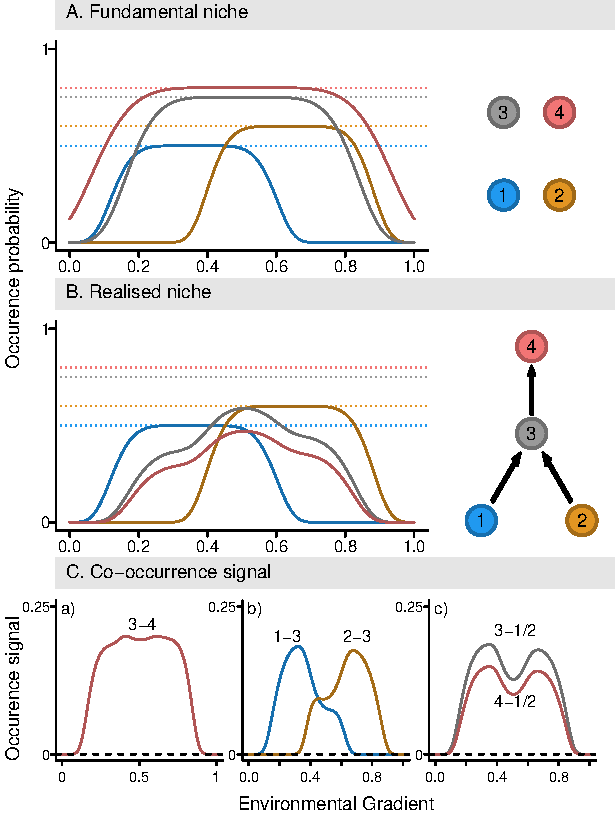
\includegraphics{../fig/figConcept.pdf}
\caption{\textbf{Probabilistic description of fundamental and realized
niches} For a three species network all the occurrence probabilities are
derived along an environmental gradient assuming that A interactions are
not limiting the distribution and B that species 3 needs at least of one
of its preys, \emph{i.e.} species 1 or 2. Horizontal dotted lines stand
for the occurrence probabilities reached at an environmental
optimum.\label{fig:box1}}
\end{figure}

\newpage

\begin{figure}[htbp]
\centering
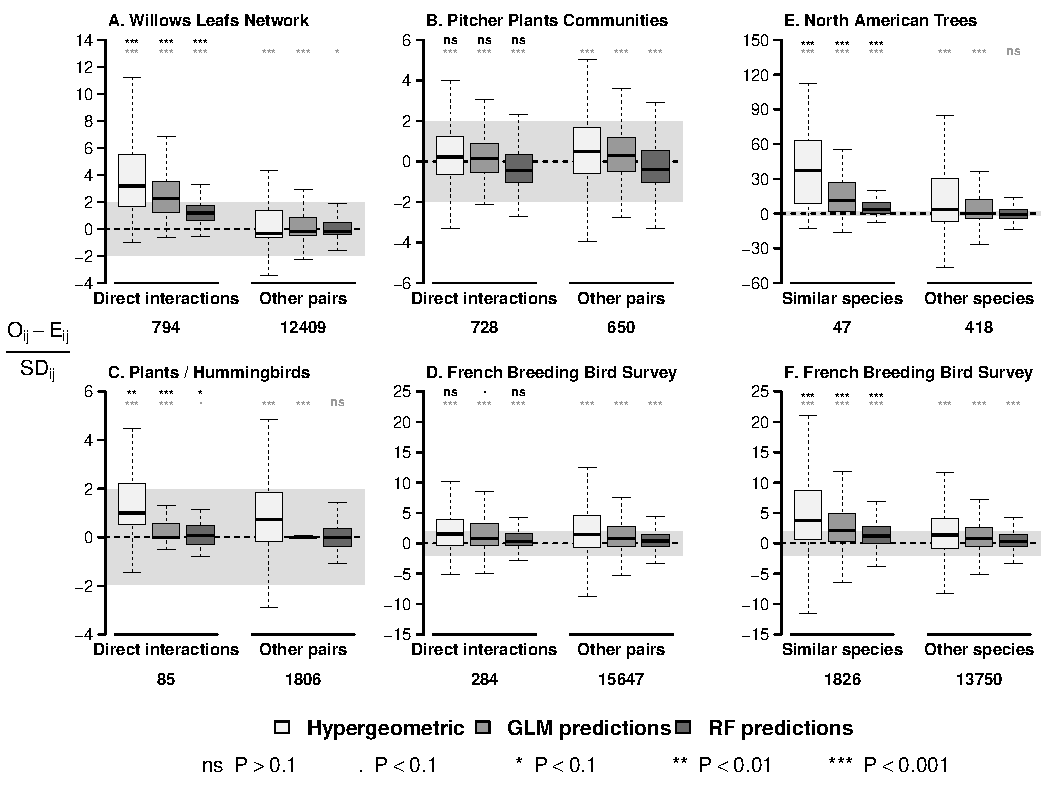
\includegraphics{../fig/figIntVsNoint.pdf}
\caption{\textbf{Co-occurrence of interacting versus not-interacting
pairs of species} Figures under each groups of boxplots indicate the
number of pairs to which the Z-score distributions refer. The light grey
rectangle corresponds to the 95\% confidence interval for the standard
normal distribution which gives insight into the proportion of pairs of
species significantly different from 0. The comparison made in panels A
to D is based on direct interactions observed. For panels E and F,
similar species are defined as the species for which the trait-based
distance is less than or equal to the lower decile of this distance
distribution. Note that outliers are not displayed. P values were
computed using the Wilcoxon rank sum test, to compare interacting versus
not-interacting Z-score distribution calculated for the three different
methods (black symbols) and to show whether the distribution is
symmetric about 0 (light grey symbols).\label{fig:synth}}
\end{figure}

\newpage

\begin{figure}[htbp]
\centering
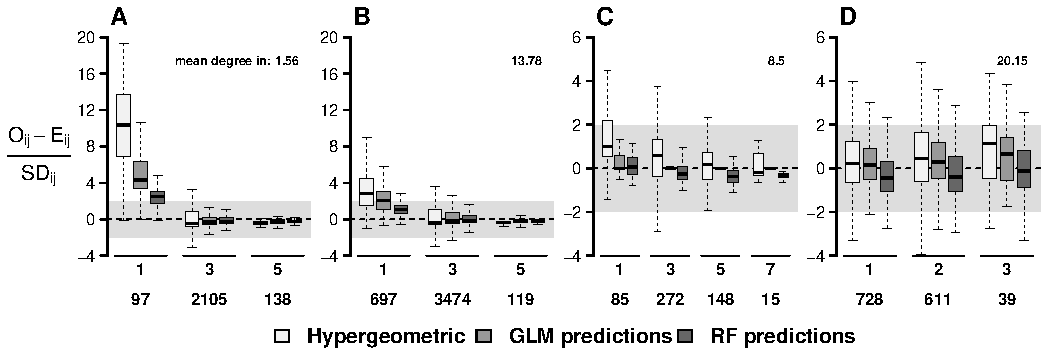
\includegraphics{../fig/figOrder.pdf}
\caption{\textbf{Co-occurrence signal decays when the shortest path
between a pair of species decay } The Z-score distribution are plotted
against the shortest path for A willows-herbivores interactions, B
herbivores-parasitoids interactions, C birds-plants interactions and D
the pitcher plants network. First figures under each grouped boxplots
indicate the shortest path associated while the figures below provide
the number of pair to which the distribution refers. Note that we used
the same y-axis for panels A and B as they regard two different kind of
interaction of the same dataset.\label{fig:shtpth}}
\end{figure}

\newpage

\begin{figure}[htbp]
\centering
\includegraphics{../fig/figdegocc.pdf}
\caption{\textbf{Co-occurrence significance decreases as the cumulated
occupancy increases} For a given species, Z-scores are averaged over the
all set species it interacts with and plotted against the joint
distribution of the same set of species. We do so for the herbivores in
the willows leafs network (panels A to C), the parasitoids in the willow
leafs network (panels D to F), the hummingbirds in the Caribbean
hummingbirds datasets (panels G to I) and all species in the pitcher
plants network that consume other species (panels J to L). The x-axis is
expressed as a log proportion of the total number of sites. Black
symbols are mean Z-scores significantly different from 0 (see SI Text).
In each panel, the dotted line represents the linear regression
\(y~ax+b\) for which the \(R^2\) is provided. The size of circles
reflects the degree of species for which the Z-score was calculated, the
relation size-degree for each row is given in the middle panel. For the
hummingbirds dataset (panels G to I), the triangle represent the values
obtained for the former distribution of a species already analyzed (see
SI text).\label{fig:degocc}}
\end{figure}

\newpage
